\chapter{Background}
\label{cha:back}

In this chapter I will cover the context of my project to allow a reader to understand the more complex parts of the report to come.\\
First I will explain the different symptoms that can be felt from hay fever and how they might be caused by different allergens.\\
I will then talk about the main data set used throughout and how I interpreted the data to produce meaninful results.\\

\section{Seasonal Allergies}
A massive 44\% of Britons suffer from at least one allergy, most of those suffering from some kind of seasonal allergy. Allergies are on the rise even with modern allergy medication improving.
\cite{mintelallergy}

\subsection{Asthma}
When talking about hay fever, most assume that it only affects the nose. However, in a study by Eur Respir J. it was found that 20.4\% of allergy sufferers also self-reported suffering from asthma\cite{rhinitis}. By 2025, asthma will represent the most prevalent chronic childhood disease and result in one of the highest health care costs, mainly due to its requirement for ongoing treatment throughout the patients life\cite{childhood}. Despite many decades of research, we do not have a complete solution to the problem. The best we can do it limit exposure, Inhale will help with this by highlighting areas with unsually high occurances of particular symptoms.

Allergy induced asthma causes day-to-day life impacting symptoms. The causes of asthma below clearly indicate allergens and traditional hay fever triggers are also related to asthma causes.\\


\begin{itemize}
  \item Allergens : including pollen, dust mites, animal fur ("dander") or feathers
  \item Airborne Irritants : including cigarette smoke, fumes and pollution
  \item Emotions : including stress or laughter
  \item Weather Conditions : including sudden changes in temperature, cold air, windy days, thunderstorms and hot, humid days
  \item Infections : particularly infections of the upper airways, such as colds and flu
\end{itemize}Adapted from \cite{urlasthmacauses}\\

As you can see, there is a huge variety of factors contributing to allergies. It would be impossible to cover all of these in my one year project. I am going to focus on Airborne Irritants and Allergens.


\section{Britain Breathing}

Britain Breathing is a Citizen Science project run by the British Society for Immunology, Royal Society of Biology and the University of Manchester Immunology Group. They collect data on seasonal allergies using a simple but effective mobile application available on Android.\\

\begin{SCfigure}
\caption{Screenshots from the data collection screen on the Britain Breathing Android app}\\
\centering
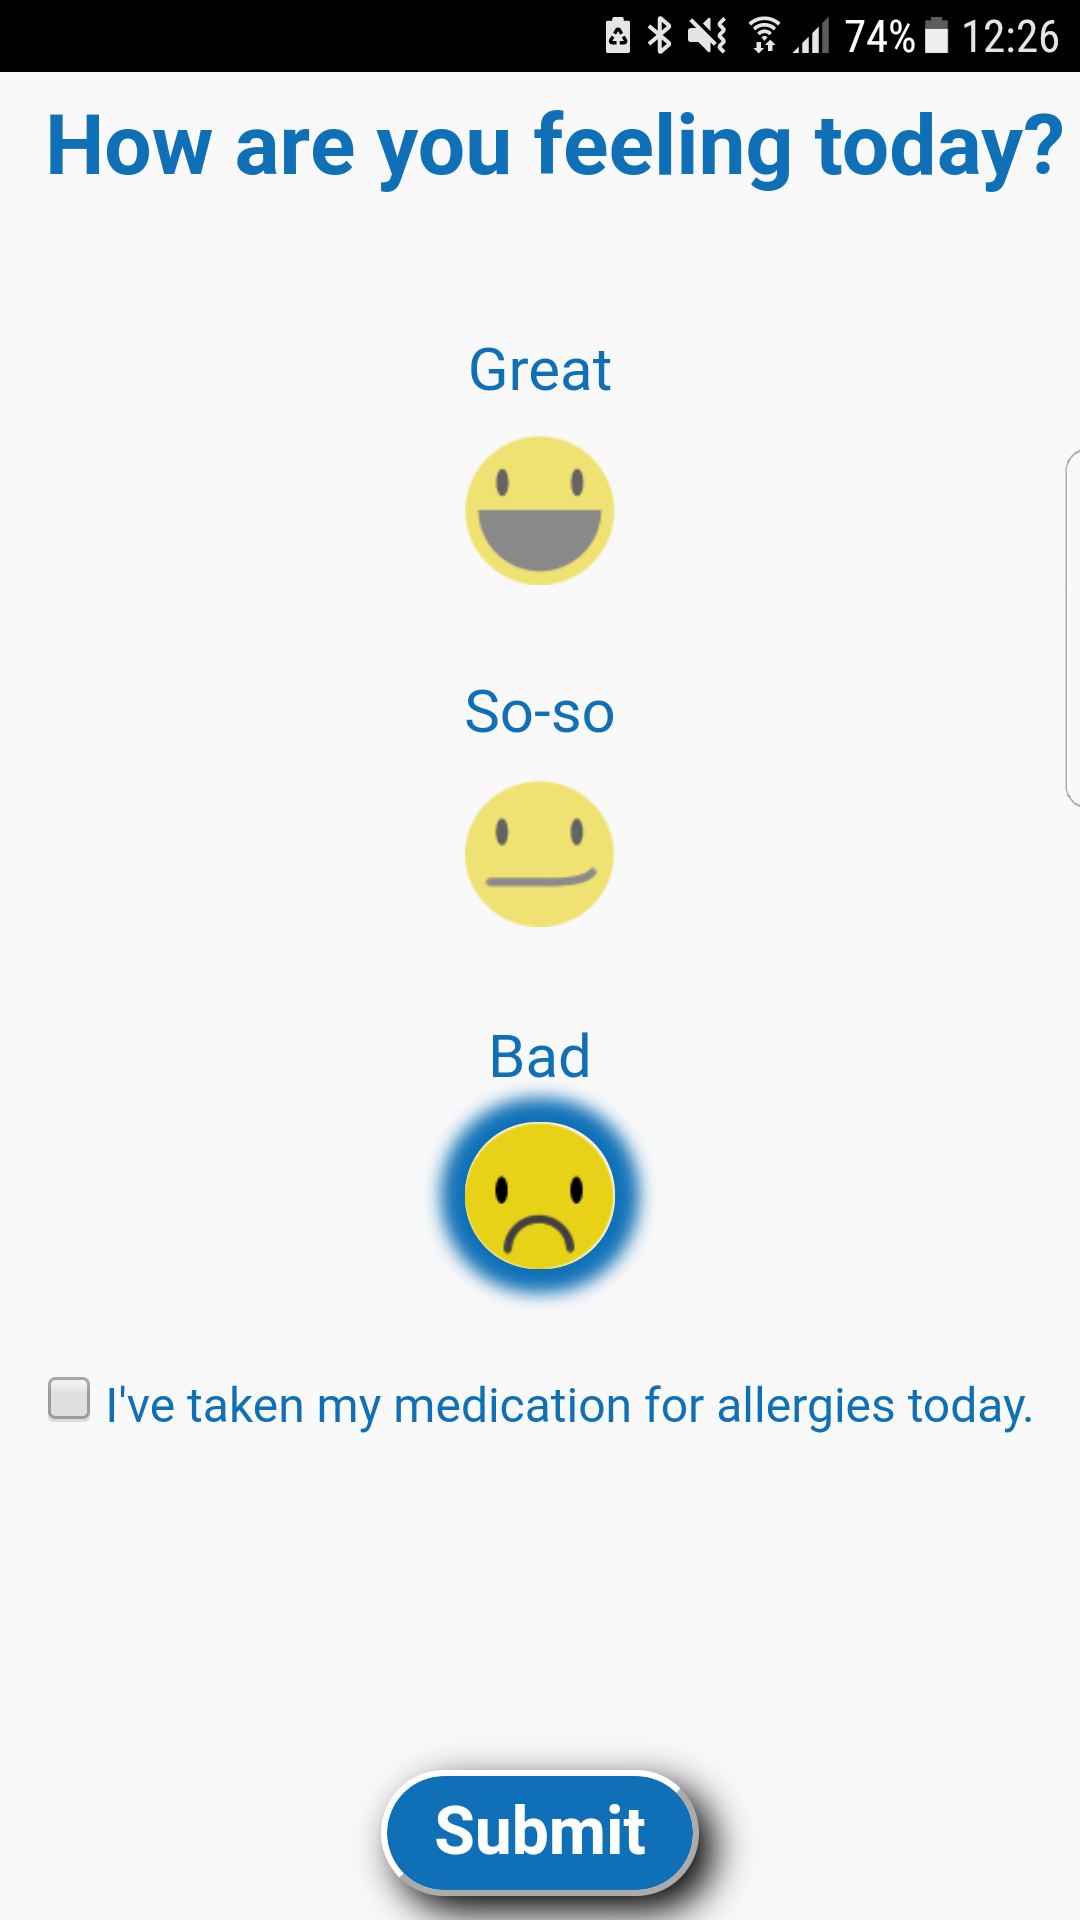
\includegraphics[width=6cm, height=8cm]{bbapp}
\centering
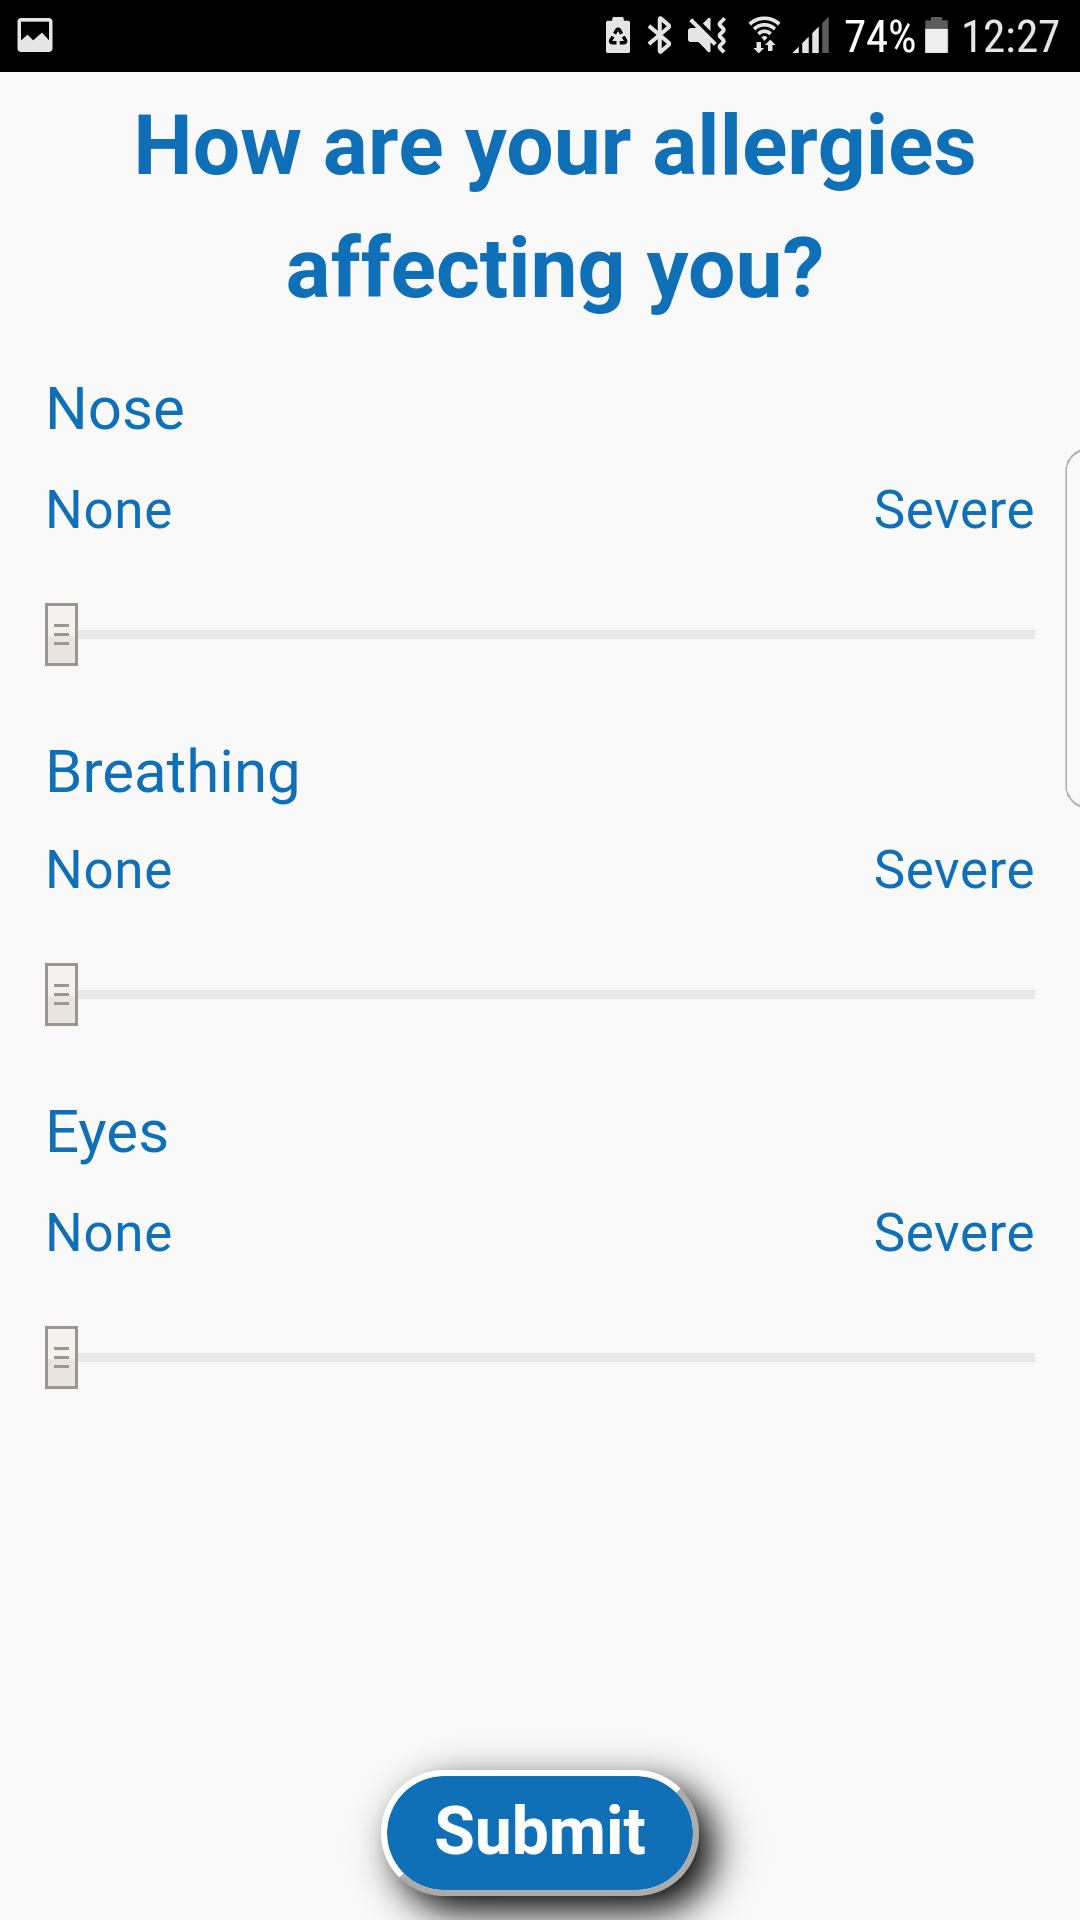
\includegraphics[width=6cm, height=8cm]{bbapp2}
\end{SCfigure}\\

Dr. Markel Vigo who is part of the Britain Breathing project was kind enough to provide me with their dataset from September 2016. This dataset contains 18,386 records from all over the UK. The data contains values that attempt to measure the severity of certain symptoms such as how bad the users nasal symptoms are. They also ask whether or not the user has taken their medication today, this field is particularly useful as it can be used as a multiplier. If someone has severe nose, eye and breathing symptoms and they have taken their medication, then this should be represented in the final visualisation as they're obviously being exposed to a significant amount of allergens.\\

See Table 2.1 for an example of the data provided by Britain Breathing.

As the data contains many different symptom areas, I will have to focus my efforts on one particular problem. Trying to cover nose, eye and breathing problems would be too much for this project. I decided to focus on the allergy score. In the Implementation chapter I will go into further detail of how I combine all of the data attributes but still keep my focus on Asthma.

Here are a couple of mathematical formulae:


A table is just like a figure. Table~\ref{wombat} uses the tabular
environment.  Environments such as tabular can be used in ordinary
text as well.
\begin{table}
\begin{center}
\begin{tabular}{|c|c|c|c|c|c|c|c|c|c}\hline\hline
Breathing&Eyes&How Feeling&Nose&Taken Meds&Asthma&Hay Fever&Latitude&Longitude\\\hline
0&0&0&0&1&1&0&54.10&-2.39\\
3&0&2&3&1&1&1&53.89&-2.79\\
3&1&0&3&1&1&1&53.24&-2.34\\\hline\hline
\end{tabular}
\end{center}
\caption{Simplified example of Britain Breathing dataset}\label{wombat}
\end{table}


\section{Existing Applications}
\label{sec:diagrams}

There are not many directly relevant applications. I think the reason for this is that in order to produce a meaningful application you need a well formed dataset. In order for a dataset to be relevant, it needs to be of a reasonable size, have a good range of locations and a diverse demographic. Without collecting data from the people directly affected it's not going to be possible to make educated conclusions on allergy hotspots.

\subsection{Britain Breathing}
Britain Breathing have a Data Visualiser on their website. It provides a simple display of the allergy data for a particular data range and a particular data value. At the time of writing this report the Visualiser is not working so I can only display a screenshot of the interface and not the actual visualisation.

\begin{SCfigure}
\caption{Britain Breathing Visualiser Interface}\\
\centering
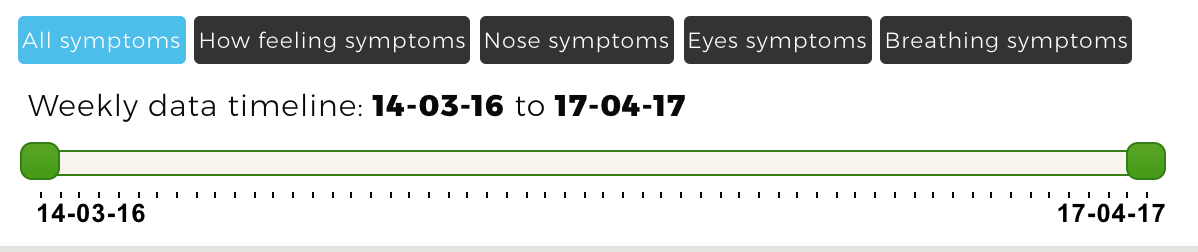
\includegraphics[width=0.75\textwidth]{bbvisinterface}
\centering
\end{SCfigure}\\

\subsection{Pollen forecast}

The closest you can get to Inhale is pollen forecast services such as Pollen.com's Allergy forecast Map. As the name suggests it only shows the pollen forecasts, and whilst this will have some correlation to the Allergy symptoms, pollen is only a small part of the problem.\\

To get a good indication of allergy symptoms, unsurprisingly, you need allergy symptom data.\\

\begin{SCfigure}
\caption{Pollen.com Allergy Forecast Map}\\
\centering
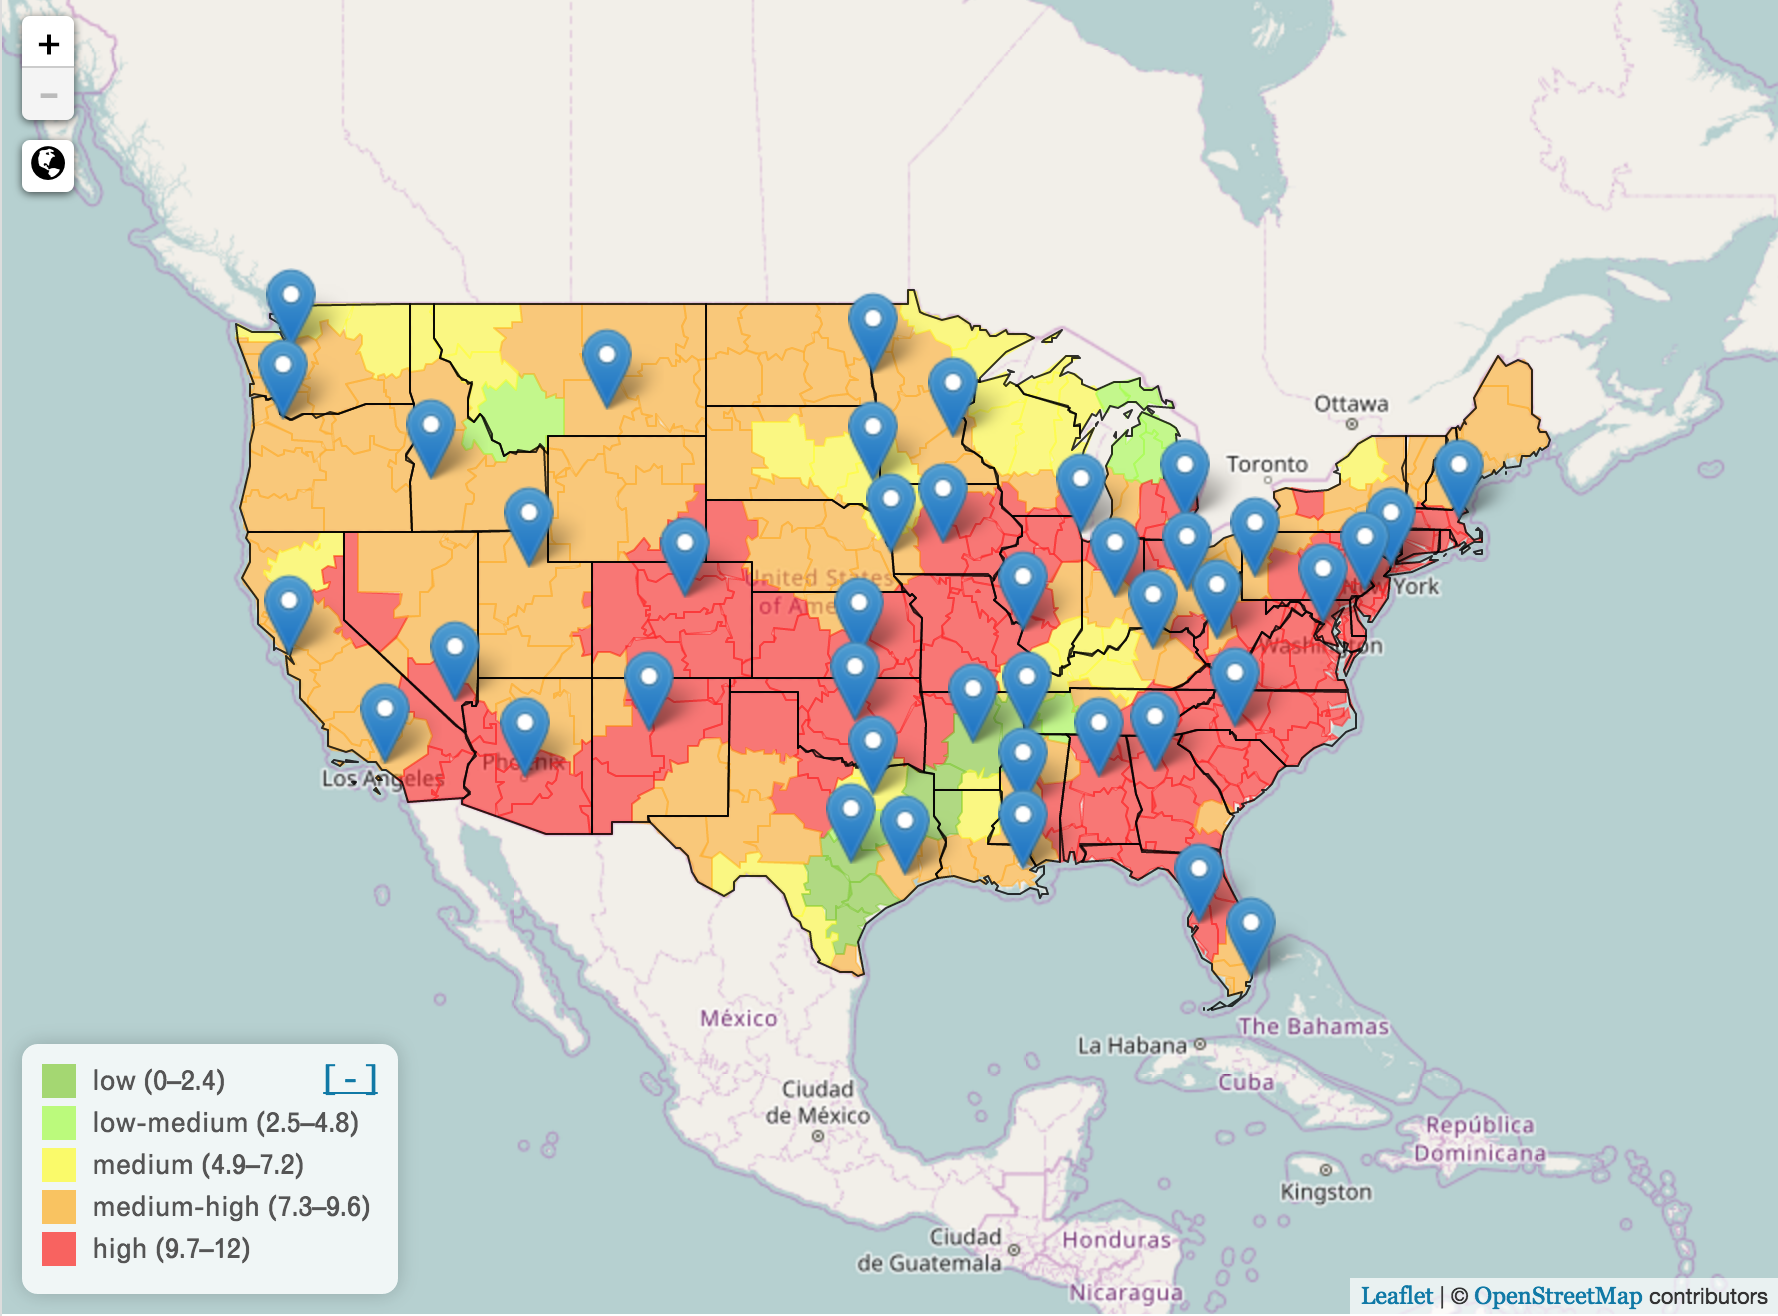
\includegraphics[width=0.75\textwidth]{pollenforecast}
\centering
\end{SCfigure}\\

% Local Variables: 
% mode: latex
% TeX-master: "report"
% End: 
